\chapter{Power management}
Il termine power management è stato usato nel corso degli anni per raggruppare problemi di diversa tipologia, ma che ruotano tutti attorno al concetto di energia.
Tra questi infatti si può includere:
\begin{itemize}
    \item Power management legata alla gestione della potenza assorbita,che si può a sua volta suddivisa in:
    \begin{itemize}
        \item Thermal Design Power, potenza termica massima che un componente può dissipare;
        \item Therm Design Current o Peak Current, legata alla massima corrente erogabile da alimentatori o dai pad dei chip; %todo: change
    \end{itemize}
    \item Thermal management, gestione temperatura dinamica o statica;
    \item Energy management, gestione della sostenibilità e del consumo di energia;
\end{itemize}

Nel contesto di questa ricerca, si farà riferimento a questa parola per abbracciare tutti e tre i concetti che essa può rappresentare, riflettendo così una visione olistica per la comprensione del problema.   

\subsection{High-Performance Computing}
Il contesto nel quale viene definito solitamente un Power Management è un sistema di computazione ad alte prestazioni, detto anche sistema HPC. Questi ultimi sono macchine computazionali composte da decine di centinaia di nodi interconnessi tra di loro da reti a bassa latenza e alta banda. 
%Ogni volta che deve essere eseguito un compito, l'utente richiede che vengano allocate delle risorse, sopra il quale far eseguire gli applicativi. Queste richieste, vengono inserite in delle code, gestite dallo scheduler di sistema %TODO:da controllare 
% che poi vanno a frammentare virtualmente e condividere il nodo in sub-clusters tra i vari utenti. %Alla fine dei vari compiti da eseguire il partizionamento delle risorse del nodo viene annullato, riportando il nodo al suo stato iniziale. L'unica parte non partizionabile del nodo sono le CPU, memorie e acceleratori.
% HPC applications typically use the Single Program Multiple Data
% (SPMD) execution model, where the same application executable
% is instanced multiple time on different nodes of the cluster; each
% instance works on a partition of the global workload and communicates with other instances to orchestrate subsequent computational steps. For this reason, a HPC application can be seen as the composition of several tasks executed in a distributed environment which exchanges messages among all the instances. Achieving high-performance communication on distributed applications in large clusters is not an easy task. The Message-Passing Interface (MPI) runtime responds to these demands by abstracting the level of network infrastructure using a simple but high-performance interface for communication that can scale up on thousands of nodes.
% Intro, cos'è il PM? 
Tutti i nodi uniti insieme, visto l'elevato numero di processori e agli acceleratori che hanno montato al loro interno offrono capacità computazioni che nei giorni nostri hanno raggiunto ordini del ExaFlops ($10^{18}$ operazioni di  Floating Point per secondo).
Visto l'aumento della densità energetica e alle magnifiche prestazioni raggiunte, la potenza necessaria per alimentare questi sistemi sta superando i 20MWatt. Se poi si considera che la maggior parte della potenza fornita, viene convertita in calore, si deve prendere in considerazione anche i consumi necessaria per tenere raffreddati questi sistemi. Infatti se non adeguati, le difficili condizioni in cui lavorano comportano grandi inefficienze in termini di energia, che si traducono anche in degradazioni di prestazioni computazionali. 
Considerando tutto, ai centri che ospitano queste macchine si devono fornire decine di MWatt di potenza per ogni exa-supercomputer che hanno installato. 
Ordini di grandezza di questo tipo non sono facilmente ottenibili e hanno costi estremamente elevati. 
%Inoltre i prezzi per garantire questi valori di Watt aumenta in modo non lineare.
Al fine di definire dei power budget, e utilizzare efficientemente la potenza richiesta si sono resi necessari strumenti situati su diversi livelli di astrazione. 
Sono nati così i primi concetti di Power Management, componenti per controllare l'utilizzo di energia utilizzando diverse strategie al fine di ridurre gli sprechi energetici e, allo stesso tempo, garantire un temperatura di funzionamento sicura.
Power Management può essere visto come un sistema composto sia da parti software che Hardware. L'insieme di questi componenti va a formare un power-stack in grado di gestire la potenza assorbita di macchine HPC.

\section{Stato dell'arte}
Per riuscire nel suo scopo, il Power-Stack deve gestire la potenza dei sistemi a diversi livelli di granularità come sistemi, singoli nodi, e singoli elementi all'interno dei nodi. Per poterlo fare, è necessario utilizzare componenti hardware accessibili principalmente tramite servizi in-band e out-of-band.
% I servizi in-band vengono forniti alle applicazioni e ai sistemi operativi in esecuzione negli elementi di elaborazione del chip e sono composti da: (i) governor dedicati alla potenza e telemetria correlata alla potenza a livello di sistema operativo; (ii) un'interfaccia dedicata per consentire alle applicazioni e ai tempi di esecuzione del modello di programmazione di specificare suggerimenti e prescrizioni per la gestione della potenza; (iii) un'interfaccia dedicata al Sistema e alla Gestione delle Risorse per supportare il capping della potenza a livello di CPU e nodo, nonché per gestire il compromesso tra Throughput ed Efficienza Energetica. I servizi out-of-band vengono forniti all'amministratore di sistema e agli strumenti di gestione del sistema tramite il Controller di Gestione della Scheda (BMC). Questi servizi consistono nella telemetria di potenza out-of-band, nel capping di potenza a livello di sistema e nella affidabilità e assistenza.

% (ii) off-chip ai Moduli Regolatori di Tensione (VRM) che alimentano il chip, gli altri componenti a bordo e il Controller di Gestione della Scheda (BMC).

\subsection{Servizi in-band} %TODO da sistemare
I servizi in-band accedono alle risorse hardware utilizzando i medesimi canali attraverso cui transitano altre forme di informazioni e comandi. In questa specifica situazione, si tratta di interfacce che richiedono al processori stessi le informazioni necessarie. Ognuno di essi è sviluppato su più livelli tra cui i cosiddetti \emph{Governors} (o governatori), i \emph{Driver} che servono a veicolare queste informazioni ed infine componenti Hardware presenti all'interno dei chip. Fondamentalmente i governors permettono monitorare e in alcuni casi di gestire alcune metriche dei processori. Tra i più famosi Governors troviamo CPUfreq\cite{TODO} (Linux)e \emph{Intel Power Governors}\cite{TODO}. \textbf{CPUFreq} è un insieme di strumenti del kernel Linux che regola e monitora la frequenza dei processori \cite{TODO}
% [https://www.kernel.org/doc/html/v4.14/admin-guide/pm/cpufreq.html]
. Può  effettuarlo sia in autonomia, in risposta al carico di sistema, sia adattarsi in risposta agli eventi ACPI oppure essere modificata manualmente dai programmi nello spazio utente. E' reso possibili tramite degli specifici driver (intel\_pstate) che comunicano con i componenti hardware sul chip. Diversamente \textbf{Intel Power Governors} utilizza le interfacce proprietarie (RAPL) con cui monitora potenza ed energia a livello di sistema.
Entrambi questi strumenti hanno necessità di componenti Hardware dedicati come i power knob (manopole per la gestione della potenza) e sensori che permettono di monitorare temperature e tensioni.
Usare i servizi in-band sono molto flessibili e permetto di operare in real-time ed in modo dinamico. Infatti interagendo con l' Hardware e passando tramite il sistema operativo, sono necessari semplici chiamate e comandi per controllare questi strumenti.


%TODO: schema power governors e power controller


\subsection{Servizi out-of-band}
Contrariamente alle interfacce in-band, le out-of-band fanno utlizzo di \emph{sidechannels} ovvero canali di accesso alternativi per ottenere le informazioni richieste. Questi oltre a non andare ad influenzare il consumo e l'utilizzo del sistema, permettono di monitorare i componenti anche quando ci sono errori ed eccezioni. Un componente tra i più famosi nell'ambito del power management è il Board Management Controller, solitamente un microcontrollore animato da sistemi embedded linux, e accessibile tramite ssh con un canale separato (solitamente provvisto di una propria interfaccia di rete e/o bus specifici). Il suo principale scopo è quello di monitorare in modo dettagliato lo stato di tensioni, temperature, ventole e prestazioni dei processori e fornire contemporaneamente servizi di power capping sia a livello di sistema che di singoli processori. 
%TODO: se vuoi spiegare esempi di bmc come opencms e aspeed astd2600
% HDEEM Estende bmc con FPGA che legge le potenze HFrequency

\section{Interfacce di alto livello}
Nel corso degli anni con l'obbiettivo di ottimizzare e automatizzare l' \emph{ottenimento} di queste informazioni sono stati sviluppati diversi software di più alto livello che utilizzano sia strumenti in band che out of band per gestire il power management. Tra questi rivediamo i punto famosi: \emph{Variorum} (LLNL), \emph{GEOPM} (Intel)\cite{GEOPM}, e \emph{HDEEM} (Atos)\cite{HDEEM}. Tutti questi vogliono fornire una soluzione ad un sottoinsieme di problemi gestione dell'energia piuttosto che ad un software globale di Power Management di sistemi di calcolo ad alte prestazioni.
% Additionally, have been introduced predictive analysis and machine learning\cite{MLEC} algorithms. Predictive algorithms can predict load spikes and implement precautionary measures to lower consumption, while machine learning can fine-tune energy management strategies using historical and real-time data. Moreover, predictive algorithms often based on ML models are essential for estimating the workload sensitivity to a given power reduction or operating point selection. Indeed, it is essential for energy management and power management algorithm to reason on an implicit or explicit performance model.

% All these solutions represent attempts to tackle power management challenges, yet they display differing levels of compatibility. This lack highlights the urgent need for a comprehensive interoperability framework. These tools, though efficacious for specific use cases, often fail to cohesively integrate and cooperate due to varying interfaces and implementations.

\section{Modello di power stack} %Componenti power stack
Con Power-Stack si intende un insieme di applicazioni software che cooperando riescono a fornire ad applicazioni, utenti e amministratori gli strumenti per un servizio di Power Management. Una volta definito il problema, e i componenti che possono essere utilizzati, è possibile definire un modello di interazione e responsabilità dei vari attori. Di seguito vengono riportati quelli che sono i ruoli necessari al fine di coordinare un sistema ad HPC dall'esecuzione di un applicativo, fino alla gestione delle tensioni. 
\begin{itemize}
    \item Workflow engine
    \item System Manager
    \item Job Manager
    \item Resource Manager
    \item Node Manager
    \item Monitor
\end{itemize}
%TODO add an example of each component

Di seguito viene riportato uno schema\ref{fig:powerstackscheme} che mostra le interazioni tra i vari attori.
\begin{figure}[H]
    \centering
    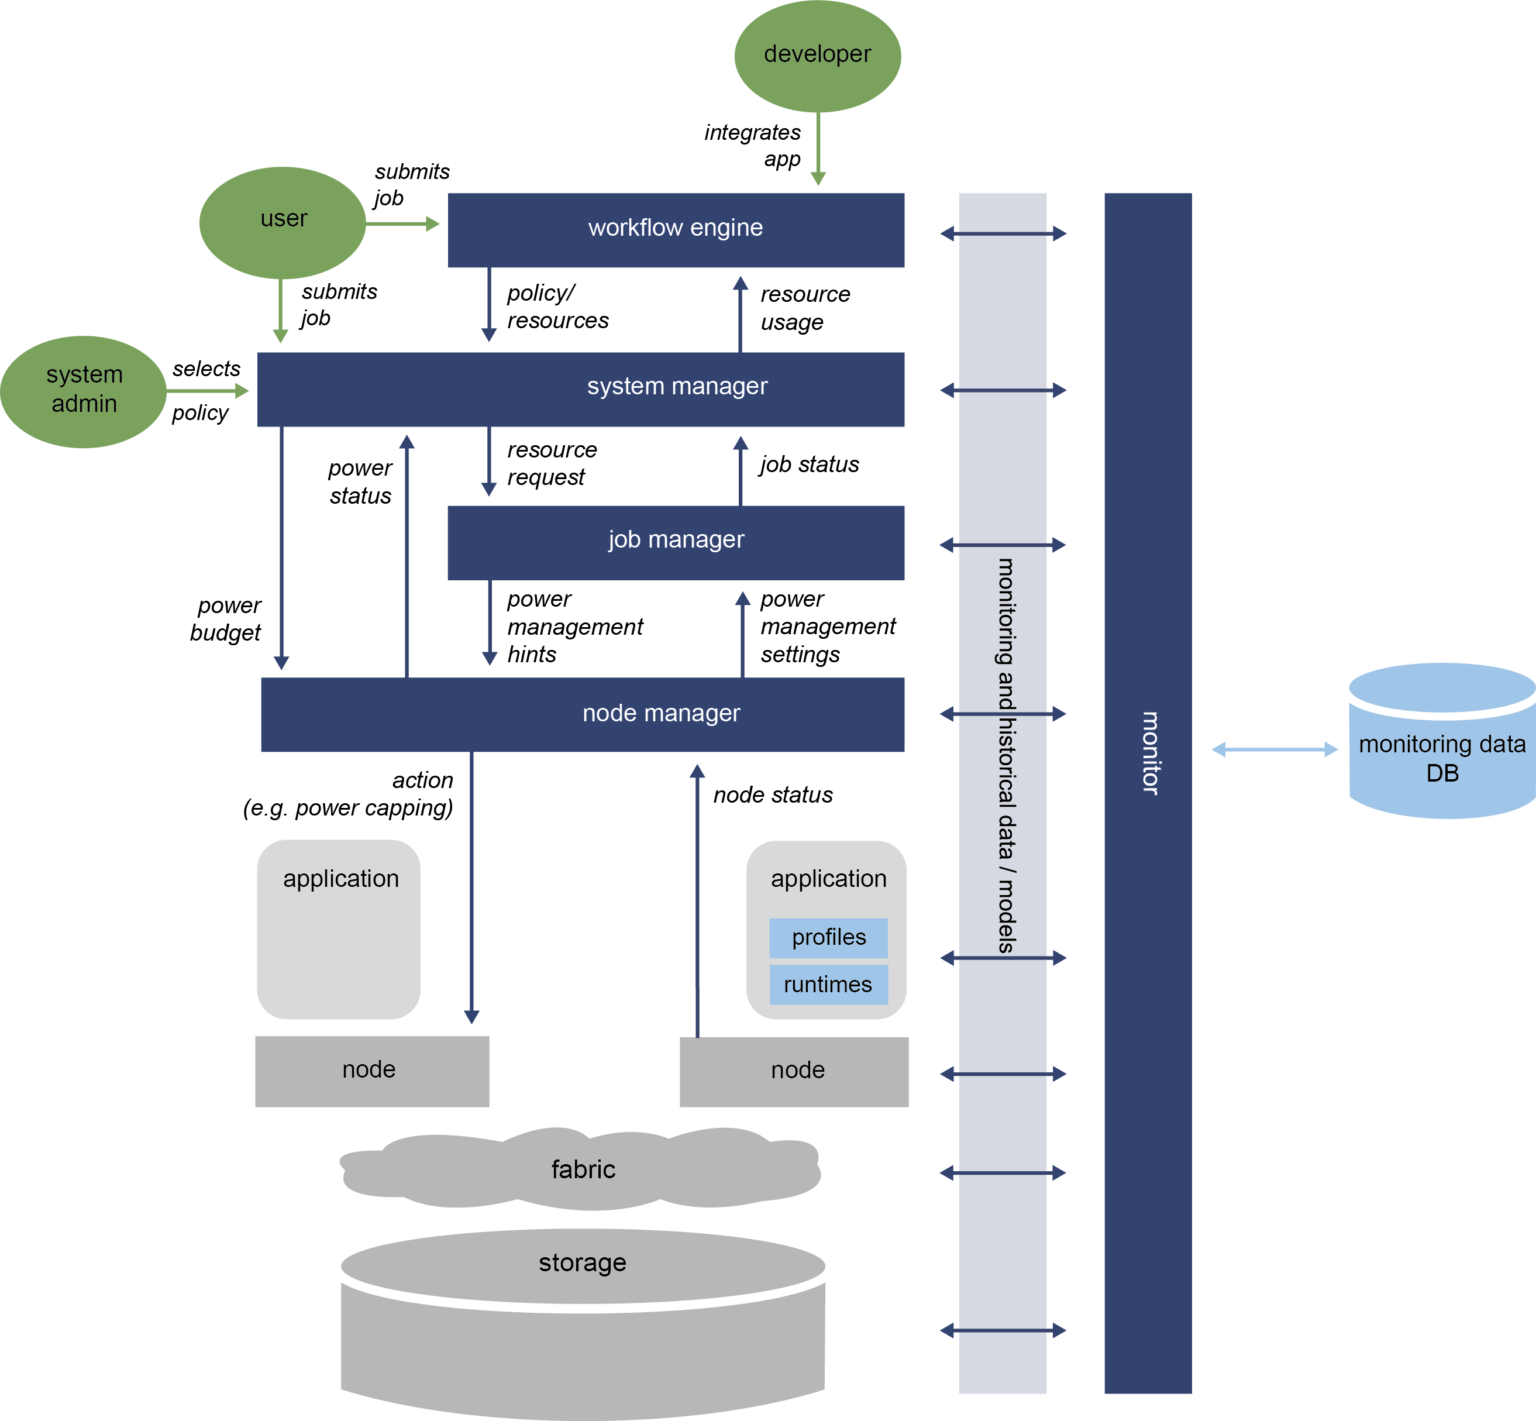
\includegraphics[width=\textwidth]{img/REGALE-Architecture-1536x1421.png}
    \caption{Modello di power stack} 
    \label{fig:powerstackscheme}
\end{figure}
\subsection{Workflow engine}
Il workflow engine analizza le dipendenze e le richieste di risorse di ogni workflow e decide dinamicamente come dividerlo negli specifici jobs che verranno assegnati al system-manager.

\subsection{Job schedulers}
Il job scheduler ha il compito di assegnare e condividere le risorse computazionali e fisice del sistema HPC, ai vari utenti che lo utilizzano. In particolare la serie di compiti che si trova a svolgere è il seguente L'utente schedula i jobs da svolgere in una o più code, definite dallo scheduler. Il Job scheduler esamina tutte le code e i job in esse contenute, e decide dinamicamente, quale sarà l'ordine di esecuzione, e il tempo massimo in cui viene assegnata una risorsa. Generalmente si cerca di ottimizzare alcune caratteristiche come il tempo di utilizzo del sistema oppure l'accesso veloce alle risorse per alcuni sottoinsiemi di jobs. Inoltre le code definite, possono avere diverse priorità o può essere ristretto l'accesso a soli alcuni utenti. I job scheduler possono condividere un nodo anche con più utenti contemporaneamente, in base all'utilizzo che devono farne. Per farlo il nodo viene allocato e diviso in partizioni virtuali, che vengo sciolte una volta finiti i job in esecuzione. Questo permette di utilizzare al massimo i componenti messi a disposizione dal sistema HPC.

\subsection{Resource Manager}
Per riuscire a svolgere questo lavoro il Job Scheduler interagisce con uno o più \textbf{Resource Manager}. Questi sono software che hanno il privilegio di gestire le risorse di un centro di calcolo. Queste risorse includono diversi componenti:
\begin{itemize}
    \item Nodi
    \item Processori
    \item Memorie
    \item Dischi
    \item Canali di comunicazione (compresi quelli di I/O)
    \item Interfacce di rete 
\end{itemize}
Per esempio quando un Job Scheduler deve eseguire un job, richiede al RM di allocare core, memorie, dischi e risorse di rete in linea con quanto il job ha necessita di essere eseguito.

Infine in alcuni casi il RM è anche responsabile di gestire elettricità e raffreddamento dei centri di calcolo.

\subsection{System Manager}
Il System Manager è un componente che riceve come input un insieme di jobs che devono essere schedulati all'interno del sistema, e in modo indicativo decide quando schedulare ogni job, su quale nodo, e con quale power budget. Successivamente vengono monitorati i dati relativi a potenza ed energia, e controlla di conseguenza i budget di potenza, e la \emph{user-fairness}

\subsection{Job Manager}
Lo scopo del job manager è quello di effettuare ottimizzazioni job-centriche considerando le prestazioni di ogni applicazioni, il suo utilizzo di risorse, la sua fase e qualsiasi interazione dettata da ogni workflow in cui è presente. In breve il job manager decide i target delle manopole del Power Management, come (i) CPU power cap, (ii) CPU clock frequency oltre ad eseguire ottimizzazione del codice.

\subsection{Node Manager}
Il node manager fornisce accesso ai controlli e monitoraggio hardware a livello del nodo. Volendo permette anche di definire delle policy di power management. Ha infine lo scopo di preservare integrità, sicurezza del nodo sia in termini informatici che fisici.


\subsection{Monitor}

Il monitor è responsabile di collezionare tutte le metriche in-band e out-of-band che riguardando prestazioni, utilizzo e stato delle risorse, potenza ed energia.
Tutto questo deve essere fatto con il minor impatto possibile sul sistema dove sta agendo, collezionando, aggregando e analizzando le metriche e dove necessario, scambiandole ad altri attori. A sua volta il \emph{Monitor} è scomponibile in tre sotto-moduli:
\begin{itemize}
    \item Gestione Firma che genera una firma che identifica univocamente il job; 
    \item Estimatore che valuta le proprità dei job o dello stato del sistema usando la firma generata precedentemente;
    \item Dashboard che fornisce le funzionalità da mostrare agli sviluppatori.
\end{itemize}


% TODO:
% To ask andrea:
% Quali di questi componenti sono out-in band?